% --------------------------------------------------------------- %
%             3. IOTA PANAUDOJAMUMAS TIEKIMO GRANDINĖSE 
% --------------------------------------------------------------- %

\section{IOTA panaudojamumas tiekimo grandinėse}



% IŠVADOS Prieš pradedant modeliuoti IOTA taikymą, reikia apsibrėžti sąlygas, kada tą apsimokėtų daryti. 2.2.2. skyriaus poskyriuose buvo analizuojamos IOTA savybės, kurias galima taikyti tiekimo grandinėse. Technologiją yra naudinga taikyti bet kurioje tiekimo grandinėje, kuri tenkina bent vieną sąlygą:
%\begin{itemize}
%    \item Atliekamos finansinės arba informacinės transakcijos. Pavyzdžiui, atsiskaitoma už paslaugas ar prekes, pranešame apie prekės atsiėmimą.
%    \item Reikalingas absoliutus duomenų nekintamumas, t.y. kad duomenų negalėtų pakoreguoti ar ištrinti absoliučiai niekas ir jie būtų prieinami amžinai.
%    \item Svarbus duomenų saugumas. Yra poreikis apsaugoti duomenis, kad prieigą prie jų turėtų tik įgaliotos šalys ir niekas daugiau.
%    \item Transportuojant krovinius atsiduriama zonose, kuriose nėra ryšio.
%    \item Reikalingi jutikliais arba kitais prietaisais pamatuojami duomenys, pavyzdžiui RFID jutiklis, matuojantis temperatūrą konteineryje.
%    \item Reikalingi jutikliais arba kitais prietaisais nepamatuojami duomenys, pavyzdžiui informacija apie stichines nelaimes.
%    \item Reikalingas automatizuotas M2M bendravimas. Pavyzdžiui, vieni elektroniniai prietaisai bendrauja ar perduoda informaciją kitiems prietaisams be papildomo žmogaus įsikišimo.
%    \item Yra pildomi fiziniai dokumentai, kuriuos svarbu išsaugoti.
%    \item Svarbus fizinių produktų ir duomenų apie juos atsekamumas. Pavyzdžiui, susiduriama su muitinėmis, kuriose vykdoma patikra.
%\end{itemize}



% --------------------------------------------------------------- %
%                   3.1. TIEKIMO GRANDINĖS ATVEJIS
% --------------------------------------------------------------- %

\subsection{Tiekimo grandinės atvejis}

Tiekimo grandinės pavyzdinis atvejis buvo kuriamas šio darbo autoriaus, remiantis kelių šaltinių pavyzdinėmis idėjomis \cite{christopher2016logistics} \cite{webber2009building} \cite{patrick2017continuous} \cite{justin2016customer}, kuriomis pasinaudojus buvo sukurta viena bendra diagrama, pavaizduota priedų skyriuje ir pažymėtas kaip priedas nr. 1. 

Diagrama nebuvo siekiama pavaizduoti realaus pasaulio tiekimo grandinės pavyzdžio\footnote{Dėl konfidencialumo priežasčių įmonės nėra linkusios skelbti oficialių savo tiekimo grandinių modelių.}, o labiau siekta sukurti modelį, apimantį kuo daugiau skirtingų tiekimo grandinės fazių ir etapų, kad tai leistų geriau atskleisti IOTA technologijos panaudojamumą. Autoriaus nuomone, modelis galėjo būti dar detalesnis, tačiau tai nebūtinai atspindėtų norimos perteikti esmės.

Šis teikimo grandinės atvejis vaizduoja supaprastintą vaisių tiekimo grandinę nuo sėklų įsigijimo iki kliento vaisių įsigijimo prekybos centre. Tiekimo grandinė išskaidyta į 15 diskrečių etapų, kurių kiekvienas aprašytas toliau:
\begin{enumerate}
    \item Ūkininkas superka sėklas iš tiekėjo. Prieš tai yra sudaromas raštiškas kontraktas tarp sėklų tiekėjo ir ūkininko, kad už tam tikrą kainą ūkininkas gaus tam tikrą kiekį sėklų. Be to, sutartyje gali būti papildomų sąlygų, jei sėklų tiekėjas laiku neturės sėklų arba jų kokybė neatitiks keliamų standartų.
    \item Ūkininkas nurenka pasėtą derlių. Ūkininkas pasėja vaisių sėklas, sudaro tinkamas sąlygas jų auginimui, naudoja specialias trąšas ir atėjus laikui užaugintus vaisius nurenka ir sandėliuoja.
    \item Ūkininkas parduoda derlių supirkėjui. Pardavimas vyksta pagal iš anksto sudarytą kontraktą. Ūkininkas įsipareigoja atėjus konkrečiam terminui parduoti vaisių supirkėjui atitinkamą kiekį vaisių, atitinkančių nustatytą kokybės standartą už atitinkamą kainą.
    \item Kurjeris pakrauna vaisius į sunkvežimį. Supirkėjas samdo kurjerį iš logistikos įmonės, teikiančios transportavimo paslaugas. Supirkėjas gali šiam darbui paskirti ir savo darbuotojus, atsakingus už prekių transportavimą. Pirmuoju atveju būtų sudaromas kontraktas tarp supirkėjo ir logistikos įmonės, įsipareigojančios atgabenti nepažeistas prekes iki nustatyto termino.
    \item Vaisiai transportuojami iki fabriko.
    \item Vaisiai apdirbami (pagaminami jų sub-produktai) ir sandėliuojami. Priklausomai nuo vaisių supirkėjo veiklos srities, jis gali vaisius paruošti pardavimui, pvz. apipurkšti cheminiu produktu, suteikiantį blizgumą ar atsparumą, taip pat apdirbti juos supjaustant, panaudojant kaip sudedamąją dalį kituose produktuose ir t.t. Galutiniai produktai sandėliuojami fabriko patalpose, kol atvyks kurjeriai, atsakingi už prekių transportavimą į prekybos centrus. Su prekybos centrais yra pasirašomi kontraktai, nustatantys kokius produktus už kokią kainą vaisių supirkėjas parduos prekybos centrui.
    \item Apdirbti vaisiai pakraunami į sunkvežimį. Čia kurjeris gali būti samdomas tuo pačiu principu, kaip ir 4 etape.
    \item Vaisiai transportuojami į jūrų uostą. Jūrų uostas pagal vidines taisykles perima konteinerį ir paruošia jį pakrovimui į laivą.
    \item Vaisių konteineriai pakraunami į krovininį laivą.
    \item Krovininis laivas nuplaukia į kitą uostą.
    \item Vaisių konteineriai iškraunami į sunkvežimius. Tikėtina, kad kurjeris yra iš tos pačios logistikos kompanijos, kurios sunkvežimis nuvežė konteinerį į pirmąjį jūrų uostą.
    \item Sunkvežimiai išvežioja vaisius į skirtingas šalis. Iki pasiekiant kitos valstybės sieną, kur kurjeris susiduria su muitine.
    \item Muitinėse patikrinami kroviniai. Priklausomai nuo valstybės, už krovinio įvežimą į šalį, gali būti taikomi skirtingi mokesčiai, o kroviniui taikomos skirtingos taisyklės ir standartai. Už atsiskaitymą su muitine yra atsakingas prekybos centras, norintis įsivežti prekes. Atlikus visas būtinas procedūras muitinė išduoda specialų leidimą.
    \item Vaisiai išvežiojami į prekybos centrus.
    \item Vaisiai parduodami galutiniams pirkėjams.
\end{enumerate}



% --------------------------------------------------------------- %
%   3.2. TIEKIMO GRANDINĖS ATVEJIS PRITAIKIUS IOTA TECHNOLOGIJĄ
% --------------------------------------------------------------- %

\subsection{Tiekimo grandinės atvejis pritaikius IOTA technologiją}

Šiame skyriuje autorius pateikia pavyzdinį tiekimo grandinės modelį pritaikius IOTA technologijos savybes. Kiekvienas papildytas panaudojimo atvejo etapas arba etapai aprašyti atskirai poskyriuose, pateikiant diagramą su kiekvieno punkto detaliu aprašymu.



% --------------------------------------------------------------- %
%                       3.2.1 PIRMAS ETAPAS
% --------------------------------------------------------------- %

\subsubsection{Pirmas etapas}

Pirmojo etapo papildytas modelis, „Ūkininkas superka sėklas iš tiekėjo“ (žr. 12 pav.):
\begin{enumerate}
    \item Tarp sėklų pardavėjo ir ūkininko yra sudaromas kontraktas, kad už tam tikrą sumą tam tikru metu ūkininkas galės įsigyti tam tikrą kiekį sėklų. Kontraktas pasirašomas ūkininko ir sėklų tiekėjo, o elektroninė sandorio versija užšifruojama raktu ir gautas šifras patalpinamas į IOTA raizginį. Abi šalys gauna dokumento kopiją ir šifro raktą. Niekas iš IOTA tinklo narių, išskyrus abi kontrakto šalis, negali peržiūrėti kontrakto turinio. Kontrakto šalys gali įrodyti turimos kontrakto kopijos autentiškumą užšifruodami šią kopiją ir patikrindami gauto šifro reikšmę su raizginyje esančiu šifru. Be to, tai apsaugo nuo dokumento padirbimo arba praradimo jį pametant. 
    \item Sėklų tiekėjas IOTA raizginyje sukuria MAM kanalą, kurį užsiprenumeruoja ūkininkas. Kanalas yra privatus, todėl sėklų tiekėjas prieš tai perduoda specialų raktą ūkininkui, kuris leidžia apsisaugoti, kad duomenų nematytų pašaliniai asmenys. Kanalu perduodami duomenys rašomi į raizginį, o ūkininkas realiu laiku gali stebėti sėklų būseną, pavyzdžiui lokaciją, sandėliavimo sąlygas ir pan.
    \item Sėklų tiekėjas pristato sėklas ūkininkui, o ūkininkas atlieką finansinį pavedimą tiekėjui.
\end{enumerate}

\begin{figure}[H]
    \centering
    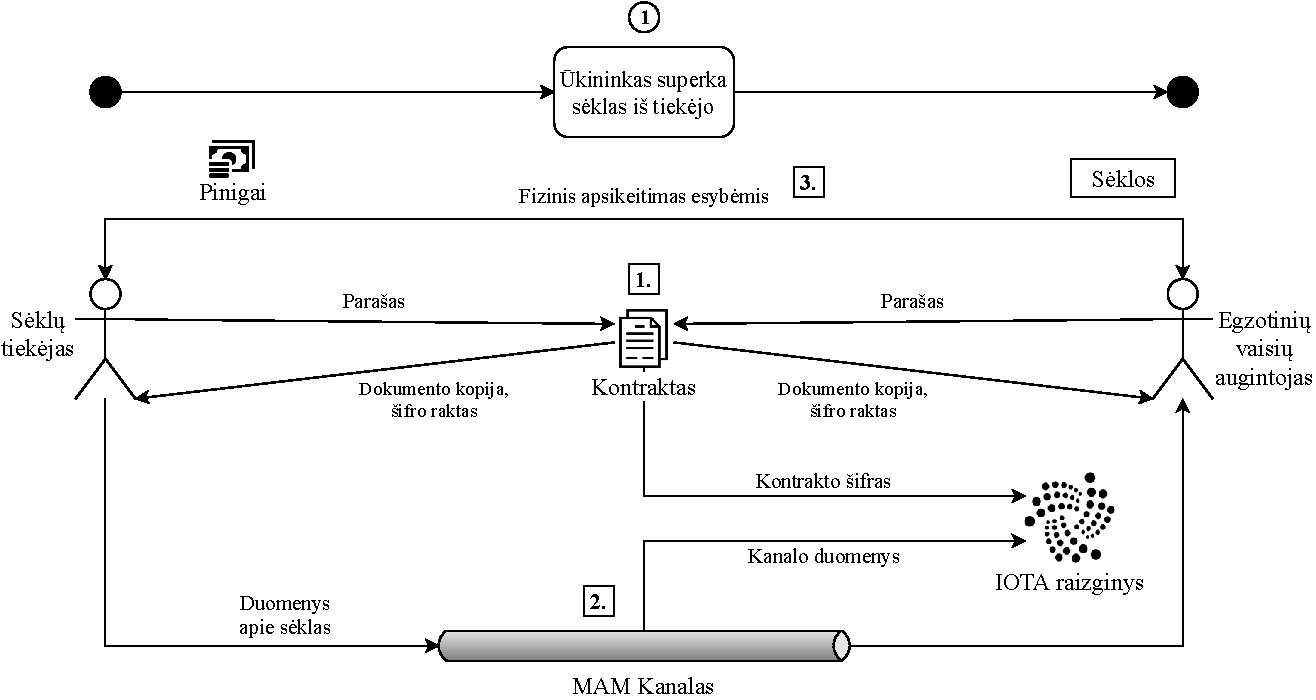
\includegraphics[scale=0.7]{images/iota-usecase-1}
    \caption{Panaudojimo atvejo 1 etapas}
\end{figure}



% --------------------------------------------------------------- %
%                       3.2.2 ANTRAS ETAPAS
% --------------------------------------------------------------- %

\subsubsection{Antras etapas}

Antrojo etapo papildytas modelis, „Ūkininkas nurenka pasėtą derlių“ (žr. 13 pav.):
\begin{enumerate}
    \item Iš pradžių ūkininkas inicijuoja privatų MAM kanalą, kuriuo siųs duomenis potencialiems derliaus supirkėjams. Ūkininkas perduoda kanalo prenumeratos raktą supirkėjui.
    \item Ten, kur yra pasodintos sėklos, pastatomi RFID jutikliai. Šie jutikliai siunčia kanalu duomenis apie vaisių auginimo sąlygas: drėgmę, temperatūrą ir kt. Jutiklius galima būtų sukonfigūruoti, kad kiekvienas atskirai siųstų duomenis į MAM kanalą, arba perduotų duomenis į ūkininko centralizuotą sistemą, kuri perimtų duomenų publikavimą.
    \item Esant poreikiui, specialūs IOTA orakulų rolę prisiėmę inspektoriai gali atlikti patikrą, ar RFID siunčiami duomenys nėra klastojami ir savo matavimus taip pat patalpinti IOTA raizginyje. Specialūs orakulai galėtų prisidėti ir prie kitų reikalavimų laikymosi patikros. Pavyzdžiui, ar ūkininkas auginimo metu neteršia aplinkos, nėra darbinami vaikai ir t.t. Orakulai gali prisidėti ir prie draudimo įmonių veiklos. Esant sausrai ir ūkininkui nepristačius pakankamai derliaus, draudimo kompanijos, gavusios patvirtinimą iš orakulų apie stichinę nelaimę, galėtų padengti ūkininkų nuostolius. Orakulų turėtų dalyvauti kuo daugiau, šitaip užtikrinant, kad daugumos jų parodymai yra objektyvūs ir sutampa. Be orakulų būtų sunku nustatyti, ar RFID duomenys, kuriuos teikia ūkininkas yra nepadirbti.
\end{enumerate}

\begin{figure}[H]
    \centering
    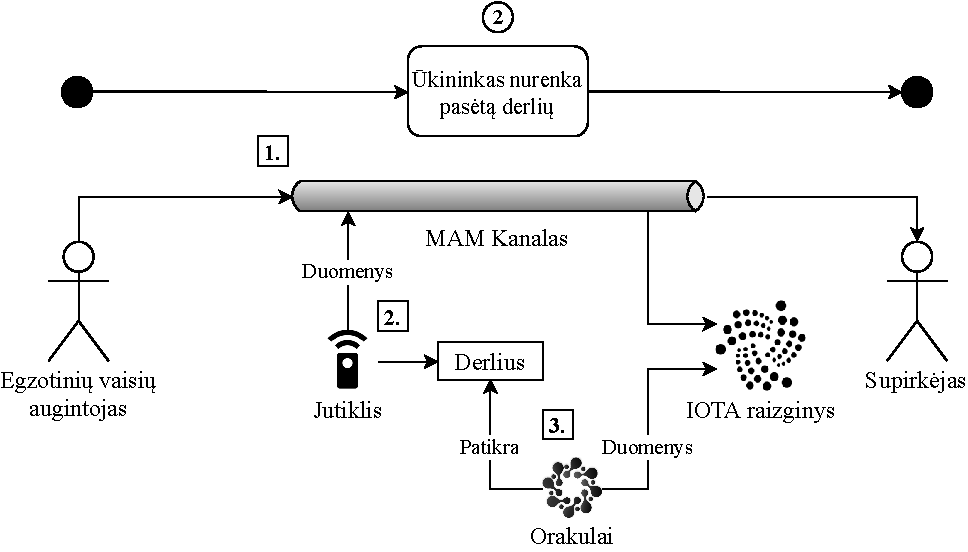
\includegraphics[scale=0.7]{images/iota-usecase-2}
    \caption{Panaudojimo atvejo 2 etapas}
\end{figure}



% --------------------------------------------------------------- %
%                       3.2.3 TREČIAS ETAPAS
% --------------------------------------------------------------- %

\subsubsection{Trečias etapas}

Trečiasis etapas, „Ūkininkas parduoda derlių supirkėjui“, yra beveik identiškas pirmajam atvejui. Šiuo atveju kontraktas tarp ūkininko ir supirkėjo gali būti sudaromas prieš 2, o esant poreikiui ir prieš 1 etapą tam, kad būtų galima paprastai sekti įsipareigojimų vykdymą.

Svarbu pabrėžti, kad sutarčių ir kontraktų gali būti daugiau nei vienas. Į IOTA tinklą tiekimo grandinės nariai gali įkelti neribotą kiekį bet kokio tipo svarbių dokumentų.



% --------------------------------------------------------------- %
%                3.2.4 KETVIRTAS IR PENKTAS ETAPAI
% --------------------------------------------------------------- %

\subsubsection{Ketvirtas ir penktas etapai}

Ketvirtojo ir penktojo etapų modelis, „Kurjeris pakrauna vaisius į sunkvežimį“ ir „Vaisiai transportuojami iki fabriko“ (žr. 14 pav.):
\begin{enumerate}
    \item Pakrovęs vaisius į sunkvežimį kurjeris sukuria MAM kanalą šitaip patvirtinantis perėmęs krovinį ir perimantis atsakomybę už jį\footnote{Paprastai kaskart atlikus transakciją perduodant krovinį, kartu perduodama ir atsakomybė už jį. Tai reiškia, kad krovinį perimanti šalis turi patikrinti krovinio būklę ir su kroviniu susijusius dokumentus, kad galėtų atrasti pažeidimo priežastį ir kaltininką.}. MAM kanalą prenumeruoja fabrikas (supirkėjas).
    \item Į MAM kanalą yra perduodami duomenys iš RFID įrenginio apie sunkvežimyje esančio krovinio sąlygas ir sunkvežimio lokaciją. Fabrikui\footnote{Šiame panaudojimo atvejyje fabrikas priklauso supirkėjui.} tai yra naudinga, nes fabrikas gali reaguoti į vaisių atvežimą, pasiruošti jam. Be to, jei vaisiai vėluotų, dingtų bei būtų pristatyti pažeisti arba neatitinkantys kokybės, būtų aišku, kur incidentas įvyko ir kas yra už tai atsakingas.
    \item Vaisiai pristatomi į fabriką, kur yra perduodama atsakomybė už juos.
\end{enumerate}

\begin{figure}[H]
    \centering
    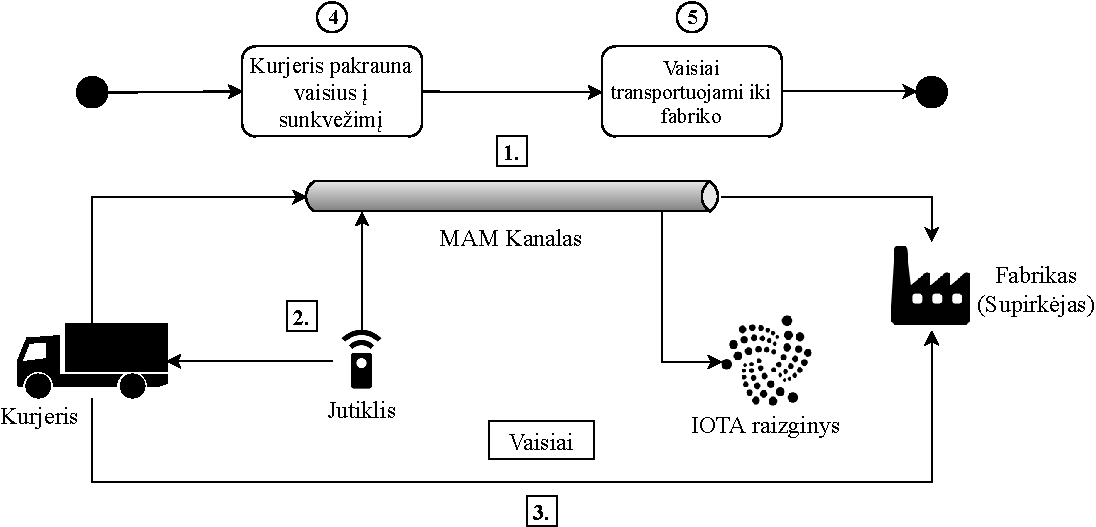
\includegraphics[scale=0.7]{images/iota-usecase-4-5}
    \caption{Panaudojimo atvejo 4 ir 5 etapai}
\end{figure}



% --------------------------------------------------------------- %
%                       3.2.5 ŠEŠTAS ETAPAS
% --------------------------------------------------------------- %

\subsubsection{Šeštas etapas}

Šeštojo etapo modelis, „Vaisiai apdirbami (pagaminami jų sub-produktai) ir sandėliuojami“ (žr. 15 pav.):
\begin{enumerate}
    \item Kaip ir pirmajame panaudojimo atvejo etape, yra sudaromas kontraktas. Fabrikas (supirkėjas) susitaria su prekybos centru, kad už tam tikrą sumą tam tikru metu bus parduotas tam tikras kiekis perdirbtų arba paruoštų vaisių. Kontraktas pasirašomas abiejų šalių, o elektroninė versija užšifruojama raktu ir gautas šifras patalpinamas į IOTA tinklą \footnote{Kontraktas gali būti sudarytas gerokai anksčiau, pavyzdžiui prieš 1 arba 2 etapą.}. Niekas iš IOTA tinklo narių, išskyrus abi kontrakto šalis, negali peržiūrėti kontrakto turinio. Kontrakto šalys gali įrodyti turimo kontrakto teisiškumą užšifruodami šią kopiją ir patikrindami gauto šifro reikšmę su raizginyje esančiu šifru.
    \item Fabrikas sukuria privatų kanalą, kurį prenumeruoja prekybos centrai\footnote{Jeigu krovinius transportuoja samdomi kurjeriai iš logistikos įmonių, kanalu duomenys gali būti siunčiami ir šiems atstovams, t.y. koks krovinių tipas, kada krovinys paruoštas transportavimui ir t.t.}. Kanalu fabrikas perduoda informaciją apie tai, kokie produktai kuriami, kurioje gamybos stadijoje šie produktai yra einamuoju momentu, kokiais standartais vadovaujantis apdirbami ir t.t.
    \item Fabrike įtaisyti RFID jutikliai kanalu taip pat perduoda informaciją, tokią kaip gamybos sąlygas skirtinguose etapuose.
    \item Esant poreikiui inspektoriai, kitaip orakulai, gali patikrinti tiek 2, tiek 3 žingsnyje fabriko teikiamą informaciją ir patalpinti į IOTA raizginį prekybos centrams pasitikrinti.
\end{enumerate}

\begin{figure}[H]
    \centering
    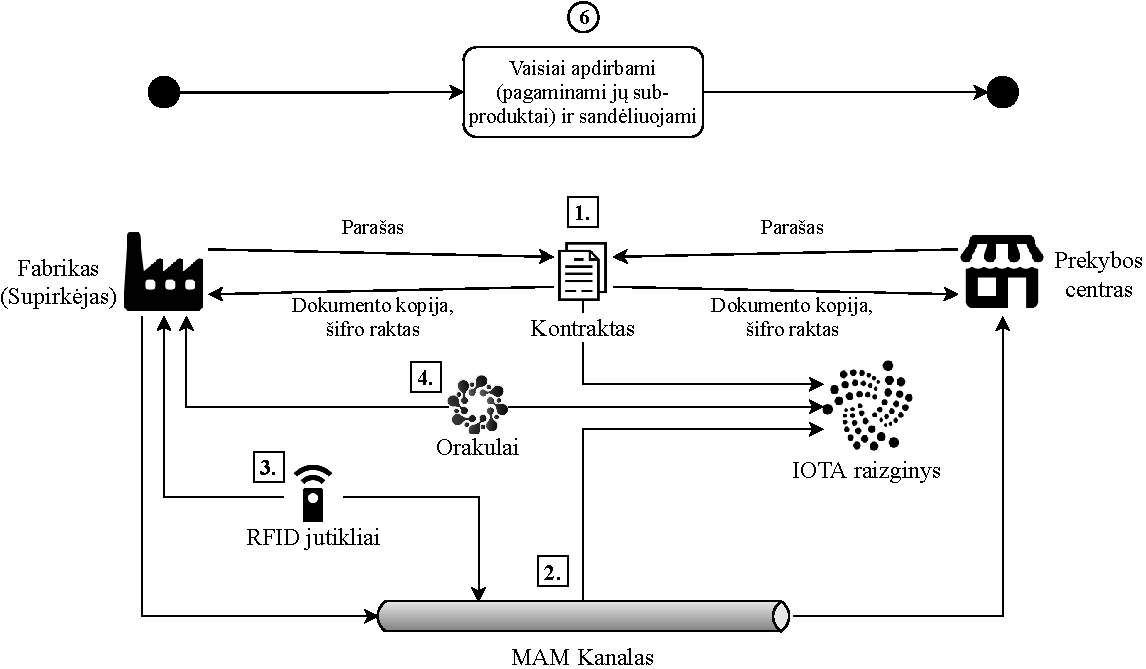
\includegraphics[scale=0.7]{images/iota-usecase-6}
    \caption{Panaudojimo atvejo 6 etapas}
\end{figure}



% --------------------------------------------------------------- %
%               3.2.6 SEPTINTAS IR AŠTUNTAS ETAPAI
% --------------------------------------------------------------- %

\subsubsection{Septintas ir aštuntas etapai}

Septintojo ir Aštuntojo etapų modelis, „Apdirbti vaisiai pakraunami į sunkvežimį“ ir „Vaisiai transportuojami į jūrų uostą“, yra beveik identiškas atitinkamai ketvirtojo ir penktojo etapų modeliui. Kurjeriui sukūrus MAM kanalą, jį prenumeruoja ne tik prekybos centras, bet ir jūrų uostas, kad būtų pasiruošta sunkvežimio atvykimui.



% --------------------------------------------------------------- %
%                3.2.7 DEVINTAS IR DEŠIMTAS ETAPAI
% --------------------------------------------------------------- %

\subsubsection{Devintas ir dešimtas etapai}

Devintojo ir dešimtojo etapų modelis, „Vaisių konteineriai pakraunami į krovininį laivą“ ir „Krovininis laivas nuplaukia į kitą uostą“ (žr. 16 pav.):
\begin{enumerate}
    \item Vaisių konteineris pakraunamas į krovininį laivą.
    \item Laivas sukuria MAM kanalą, kurį užprenumeruoja kurjeris, laukiantis krovinio jūrų uoste nr. 2. Kanalu perduodama konteinerio su vaisiais laikymo sąlygos, gaunamos iš RFID jutiklių. Laivas išplaukia iš jūrų uosto nr. 1
    \item Laivui plaukiant jūra, dingsta interneto ryšys, tačiau informacijos tiekimas nenutraukiamas ir informacijos transakcijos yra toliau atliekamos neprisijungus. 
    \item Po kiek laiko interneto ryšys grįžta ir visos iki tol siųstos žinutės atsiduria IOTA raizginyje, kurias prenumeruotojas gali gauti ir matyti iškart.
    \item Vaisiai transportuojami į jūrų uostą nr. 2.
\end{enumerate}

\begin{figure}[H]
    \centering
    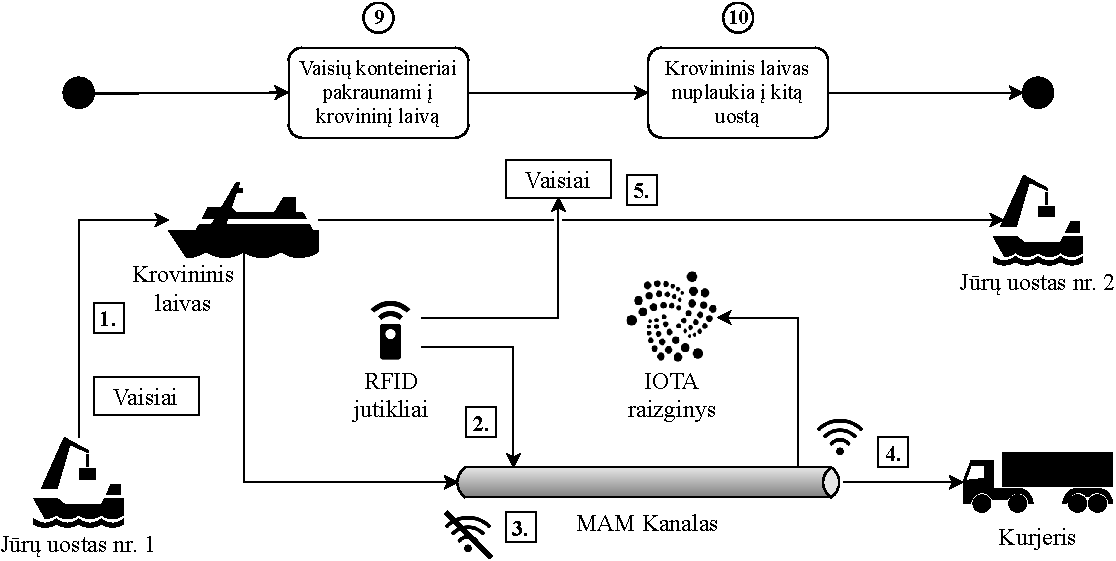
\includegraphics[scale=0.7]{images/iota-usecase-9-10}
    \caption{Panaudojimo atvejo 9 ir 10 etapai}
\end{figure}



% --------------------------------------------------------------- %
%              3.2.8 VIENUOLIKTAS IR DVYLIKTAS ETAPAI
% --------------------------------------------------------------- %

\subsubsection{Vienuoliktas ir dvyliktas etapai}

Vienuoliktojo ir dvyliktojo etapų modelis, „Vaisių konteineriai iškraunami į sunkvežimius“ ir „Sunkvežimiai išvežioja vaisius į skirtingas šalis“ (žr. 17 pav.):
\begin{enumerate}
    \item Jūrų uoste nr. 2 iškraunamas konteineris su vaisiais, kurį perima kurjeris.
    \item Kurjeris sukuria MAM kanalą, kurį užprenumeruoja Prekybos centras.
    \item Kurjeris galiausiai pasiekia kitos valstybės muitinę.
\end{enumerate}

\begin{figure}[H]
    \centering
    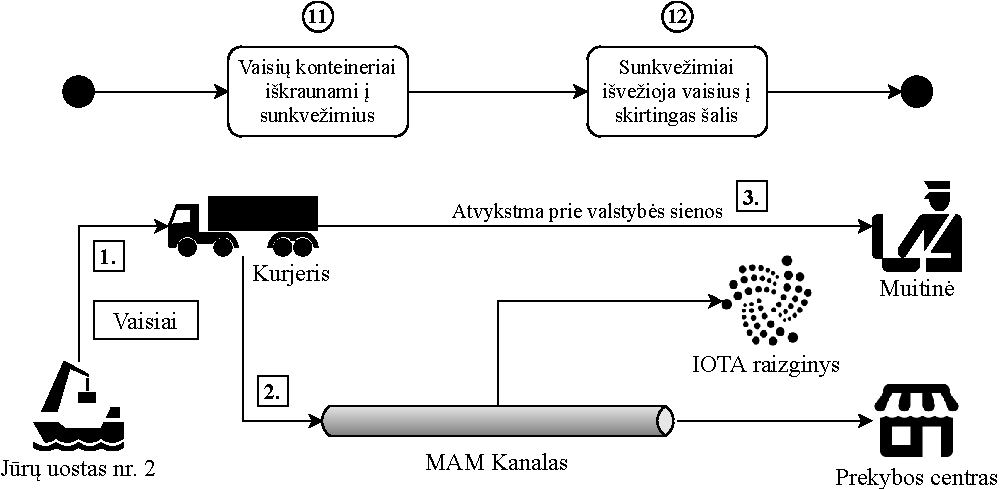
\includegraphics[scale=0.75]{images/iota-usecase-11-12}
    \caption{Panaudojimo atvejo 11 ir 12 etapai}
\end{figure}



% --------------------------------------------------------------- %
%                       3.2.9 TRYLIKTAS ETAPAS
% --------------------------------------------------------------- %

\subsubsection{Tryliktas etapas}

Tryliktojo etapo modelis, „Muitinėse patikrinami kroviniai“ (žr. 18 pav.):
\begin{enumerate}
    \item Kurjeris perduoda vaisių konteinerį muitinės darbuotojų patikrai.
    \item Muitinės darbuotojai patikrina vaisių kelionės gyvavimo ciklo informaciją IOTA raizginyje. Ši informacija leidžia muitinės darbuotojams lengvai patikrinti svarbią informaciją. Pavyzdžiui, JAV pasienio muitų įstatymas įpareigoja pateikti krovinio pirkėją, pardavėją, gamintoją, kilmės šalį ir kitus duomenis \cite{customs2018importer}. Visą šią informaciją būtų galima paprastai atsekti ir validuoti IOTA raizginyje, todėl tai galėtų sutaupyti daug laiko. 
    \item Muitinės darbuotojams neradus nieko įtartino, suteikiamas leidimas krovinį įvežti į valstybę. Leidimas taip pat gali būti įrašomas į IOTA raizginį. Vaisius transportuojanti valstybė susimoka muito mokestį (jeigu toks yra taikomas) ir toliau tęsia kelionę.
\end{enumerate}

\begin{figure}[H]
    \centering
    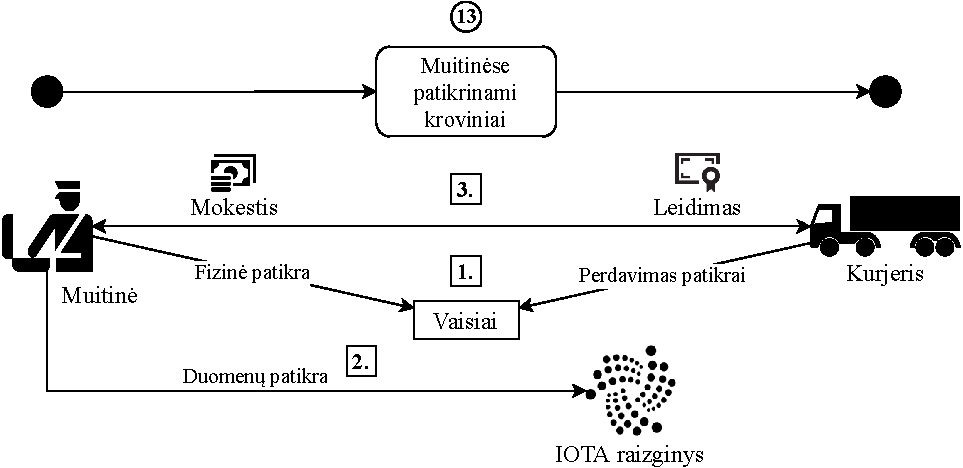
\includegraphics[scale=0.8]{images/iota-usecase-13}
    \caption{Panaudojimo atvejo 13 etapas}
\end{figure}



% --------------------------------------------------------------- %
%           3.2.10 KETURIOLIKTAS IR PENKIOLIKTAS ETAPAI
% --------------------------------------------------------------- %

\subsubsection{Keturioliktas ir penkioliktas etapai}

Keturioliktojo ir penkioliktojo etapų modelis, „Vaisiai išvežiojami į prekybos centrus“ ir „Vaisiai parduodami galutiniams pirkėjams“ (žr. 18 pav.):
\begin{enumerate}
    \item Vaisiai transportuojami į prekybos centrą, kuriame šie yra paruošiami pardavimui klientams. Ant vaisių pakuočių prekybos centras pagamina ir užklijuoja specialią informaciją savyje laikantį QR kodo lipduką.
    \item Prekybos centrų klientai nusiperka vaisių pakuotes.
    \item Pirkėjas gali įsitikinti prekybos centro pateikiama informacija, nuskenavęs ant pakuotės esantį QR kodą. Speciali programėlė galėtų leisti peržiūrėti kilmės šalį, vaisių kelionės maršrutą, vaisių auginimo, sandėliavimo ir transportavimo sąlygas, taip pat bet kokią papildomą informaciją, kurią tiekėjai gali atskleisti pirkėjui. Visa ši informacija gaunama iš IOTA raizginyje MAM kanalais bei kitais būdais patalpintos informacijos.
\end{enumerate}

\begin{figure}[H]
    \centering
    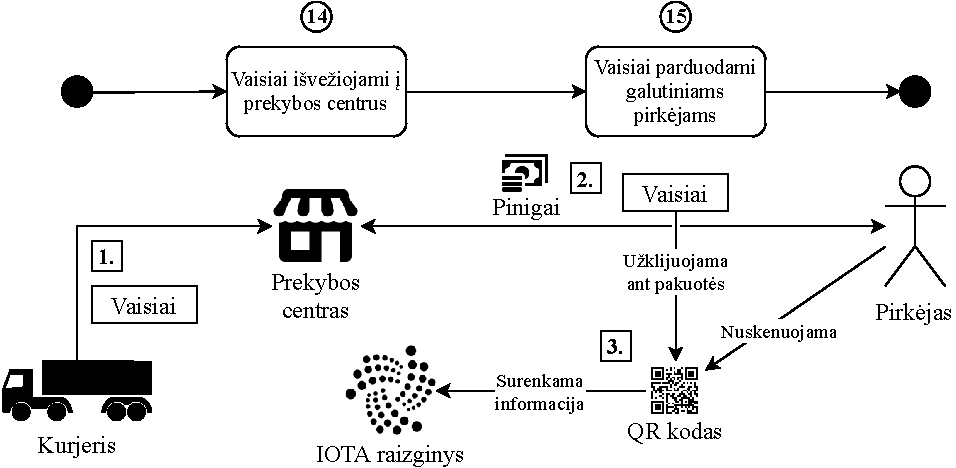
\includegraphics[scale=0.8]{images/iota-usecase-14-15}
    \caption{Panaudojimo atvejo 14 ir 15 etapai}
\end{figure}



% --------------------------------------------------------------- %
%        3.3 ALTERNATYVŪS IOTA TAIKYMAI TIEKIMO GRANDINĖJE
% --------------------------------------------------------------- %

\subsection{Alternatyvūs IOTA taikymai tiekimo grandinėje}

IOTA technologijos galimi taikymai tuo neužsibaigia.

1-12 panaudojimo atvejo etapuose buvo naudojami MAM kanalai. Tačiau šie kanalai buvo sudaromi sukuriant prenumeratos teisę tik pasroviui esančiai tiekimo grandinės šaliai. Kanalai buvo privatūs, kad informaciją būtų galima siųsti saugiai. Tačiau tiek galutiniai pirkėjai, tiek muitinės, neturėdamos specialaus rakto, informacijos turinio peržiūrėti negali. Vienas iš sprendimo būdų būtų perduoti specialų MAM kanalo prenumeratos raktą visiems pasroviui esantiems dalyviams.

Tačiau tai sukelia papildomų problemų. Skirtingų šalių yra daug: tiesioginiai klientai, netiesioginiai klientai, galutiniai pirkėjai, muitinės ir auditoriai. Visoms šalims reikalinga vis skirtinga informacija. Įmonė nenorėtų, kad konfidenciali informacija, skirta tiesioginiams klientams, pvz. transportavimo tvarkaraščiai arba turimas inventorius, būtų prieinamas galutiniams pirkėjams. Ir atvirkščiai, muitinėms, auditoriams ir galutiniams pirkėjams yra aktuali tik dalis informacijos iš viso srauto.

Naudojant skirtingus MAM kanalus skirstant informaciją tarp tiekimo grandinės šalių ir nustatant skirtingas prieigos teises, galima valdyti informacijos srautus (žr. 20 pav.). Kadangi tiesioginis klientas retai keičiasi, sukuriamas privatus MAM kanalas. Suvaržytieji kanalai X, Y, ir Z perduoda skirtingus duomenis atitinkamiems prenumeruotojams. Kadangi tiek auditoriai, tiek muitinė, tiek netiesioginiai klientai gali dažnai kisti, yra parenkama suvaržyta kanalų apsauga, leidžianti dinamiškai keisti prenumeruotojus. Viešas kanalas yra skirtas galutiniams pirkėjams, tačiau duomenis gali peržiūrėti bet kas, turintis prieigą prie IOTA raizginio.

\begin{figure}[H]
    \centering
    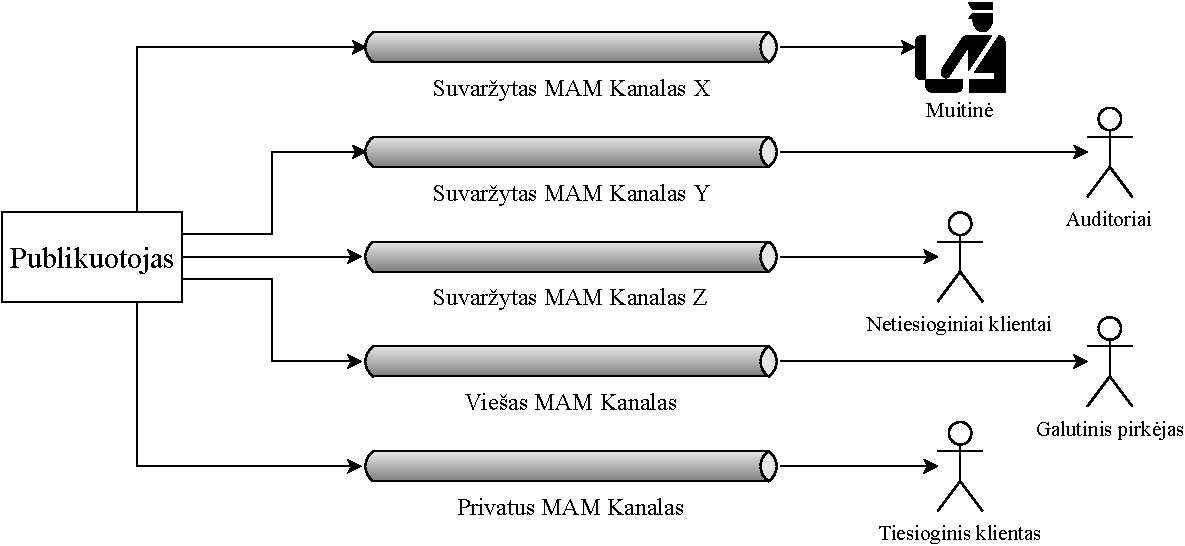
\includegraphics[scale=0.8]{images/mam-channel-flows}
    \caption{MAM kanalų srautai}
\end{figure}

Pavyzdinio panaudojimo atvejo 1, 3, 13-15 etapuose ir bet kuriame kitame etape, kuriame vienas iš žingsnių yra finansinė transakcija, galima naudoti IOTA kaip atsiskaitymo terpę. Tokiam scenarijui pavaizduoti yra tinkamas 3.2.10. poskyryje aprašomas 2 žingsnis. Šiuo atveju galutinis vartotojas, t.y. prekybos centro klientas perka vaisių pakuotę, už kurią kasoje atsiskaito egzistuojančia valiuta\footnote{Pavyzdžiui, eurais arba doleriais.} bankine kortele. Finansine transakcija pasirūpina bankas, o tai, kaip jau buvo minima 2 skyriuje, kelia įvairių rizikų.

Tačiau technologijai įsigalėjus klientas galėtų atsiskaityti kriptovaliuta IOTA raizginyje (žr. 21 pav.). Turėdamas savo sąskaitą klientas pervestų kriptovaliutą į prekybos centro sąskaitą tiesiogiai ir ši transakcija būtų iškart įrašoma į IOTA raizginį. Tai reiškia, būtų išvengiama tarpininko, šiuo atveju banko. Tokie atsiskaitymai būtų galimi ir didesniais mastais, pavyzdžiui, milijoniniai sandoriai tarp verslo šalių. Žinoma, tam reikėtų visuotinio technologijos ir kriptovaliutos pripažinimo ir nusistovėjimo, nes šiuo metu jos kaina labai svyruoja\footnote{Duomenys iš: https://coinmarketcap.com. Tikrinta 2019-05-15.}.

\begin{figure}[H]
    \centering
    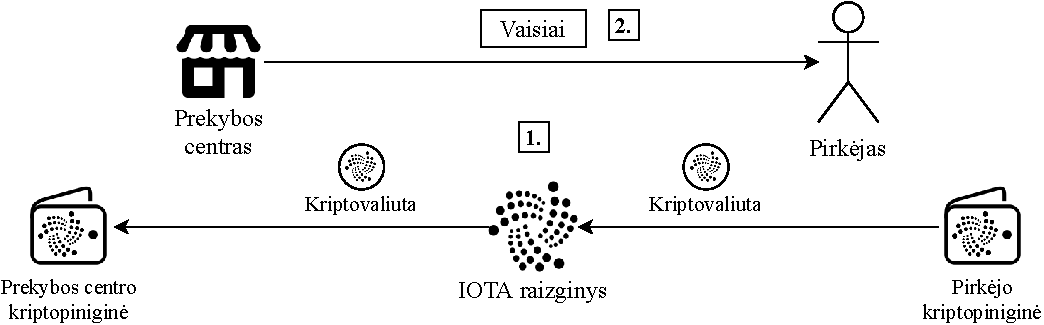
\includegraphics[scale=0.75]{images/tangle-financial-transaction}
    \caption{Finansinė transakcija IOTA raizginyje}
\end{figure}

Pavyzdinio panaudojimo atvejo 2 etape svarbų vaidmenį vaidina orakulai, įrašydami savo duomenis į IOTA raizginį. Tai leidžia patikrinti, ar ūkininko pateikiami duomenys atitinka realybę. Tačiau 2 etapo 3 žingsnį galima praplėsti naudojant orakulus ir išmaniuosius kontraktus (žr. 22 pav.): 
\begin{enumerate}
    \item Geografiniame regione, kuriame ūkininkas augina vaisius, galėtų būti įsikūrę daugybė orakulų, kurie turėtų savo temperatūros matavimo prietaisus. Šiais prietaisais jie pamatuotų temperatūrą arba kitus rodiklius.
    \item Kiekvienas orakulas perduotų savo duomenis išmaniajam kontraktui.
    \item Išmanusis kontraktas surinktų visų orakulų duomenis ir juos visus perduotų išoriniam skaičiavimų įrenginiui. Atlikus skaičiavimus įrenginys grąžintų gautą skaičiavimų rezultatą išmaniajam kontraktui.
    \item Gautus galutinius skaičiavimus ir kitą informaciją išmanusis kontraktas perduotų MAM kanalu, kurį yra užsiprenumeravęs supirkėjas.
\end{enumerate}

\begin{figure}[H]
    \centering
    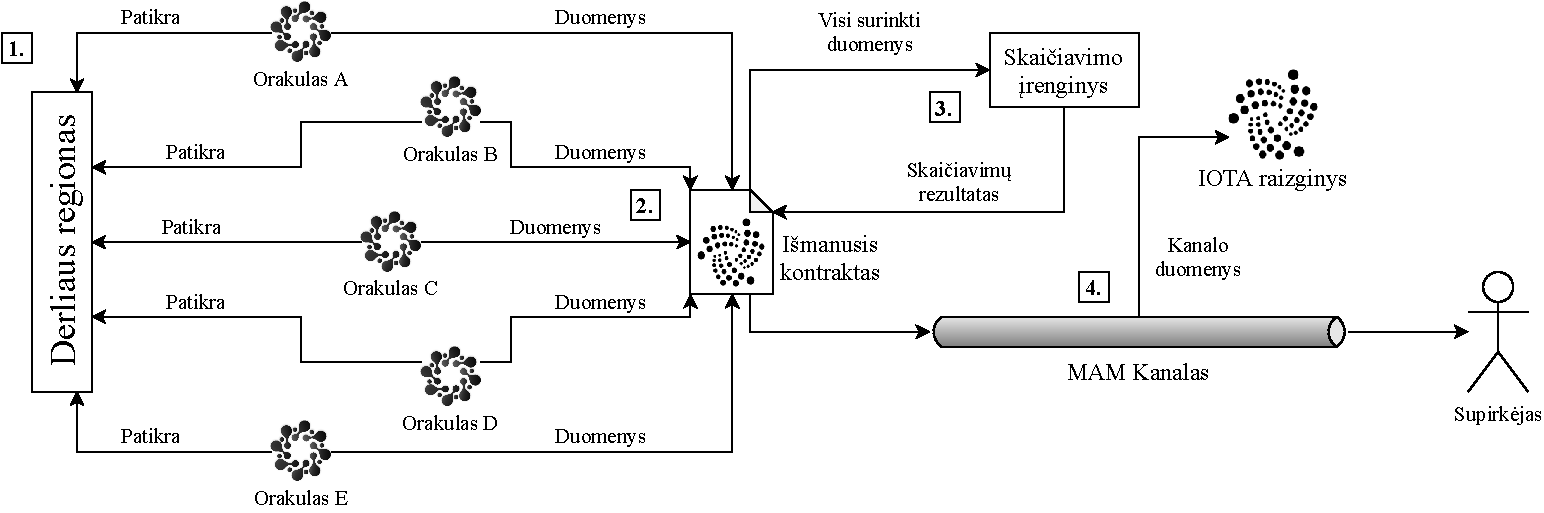
\includegraphics[scale=0.63]{images/tangle-smart-contract}
    \caption{Finansinė transakcija IOTA raizginyje}
\end{figure}